
% Este documento LaTeX fue diseñado por profesores  del Departamento de Matemáticas 
% de la Universidad de Antioqua (http://ciencias.udea.edu.co/). Usted puede modificarlo
% y personalizarlo a su gusto bajo los términos de la licencia de documentación libre GNU.
% http://es.wikipedia.org/w/index.php?title=Licencia_de_documentaci%C3%B3n_libre_de_GNU&oldid=15717448

\documentclass[serif,9pt, t]{beamer}
\setbeamertemplate{navigation symbols}{}
\addtobeamertemplate{navigation symbols}{}{
    \insertframenumber/\inserttotalframenumber
}
\setbeamercolor{navigation symbols}{fg=black}
\usetheme{Warsaw}

\usepackage[utf8]{inputenc}
\usepackage[spanish]{babel}
\usepackage{verbatim} %para comentarios multilinea
\usepackage{subfig}

\graphicspath{{figuras/}}

\newif\ifplacelogo % Para que el logo solo figure en el primer slide
\placelogotrue
\logo{\ifplacelogo
\includegraphics[scale=0.25]{logo_exactas}\fi}
\newcommand\Fontvi{\fontsize{7}{7.2}\selectfont}

\beamersetuncovermixins{\opaqueness<1>{25}}{\opaqueness<2->{15}}

\begin{document}
\title[Análisis y Detección de Correlaciones en Relevamien\ldots ]{Análisis y Detección de Correlaciones en Relevamientos Transcripcionales de Gran Escala}  
\author[Andrés Rabinovich]{Andrés Rabinovich\\{\small Director: Dr. Ariel Chernomoretz}}

\institute[Departamento de Física]{
	Departamento de Física\\	
	Facultad de Ciencias Exactas y Naturales\\
	Universidad de Buenos Aires}
\date{Marzo 2016.}


\begin{frame}
\titlepage
\end{frame}

\placelogofalse

\begin{frame}\frametitle{Contenido}
\tableofcontents
\end{frame} 

\section{Introducción} 

\subsection{Detección de correlaciones}
\begin{frame}\frametitle{Detección de correlaciones} 
\large
Queremos encontrar relaciones entre grandes cantidades de datos.\\\bigskip
Lo vamos a hacer usando métodos de agrupamiento o ``clustering''.\medskip
\normalsize
\begin{itemize}
\item Son métodos de clasificación no supervisados.
\item Consisten en agrupar elementos ``similares entre si''.
\item Permiten el descubrimiento de patrones en los datos.
\item Posibilitan obtener conclusiones sobre los datos.
\end{itemize}
\bigskip
\underline{A modo de ejemplo}\medskip

El conjunto: $\{-5, -3, -2, 2, 3\}$\medskip

Agrupado por módulo: $\{-5\}$, $\{-3, 3\}$ y $\{-2, 2\}$\medskip

Agrupado por signo: $\{-5, -3, -2\}$ y $\{2, 3\}$
\end{frame}

\subsection{Relevamientos transcripcionales de gran escala}

\subsubsection*{Transcripción y traducción}
\begin{frame}\frametitle{Transcripción y traducción (dogma central de la biología molecular)}

\begin{figure}[t]
  \centering
  \subfloat[Célula eucariota]{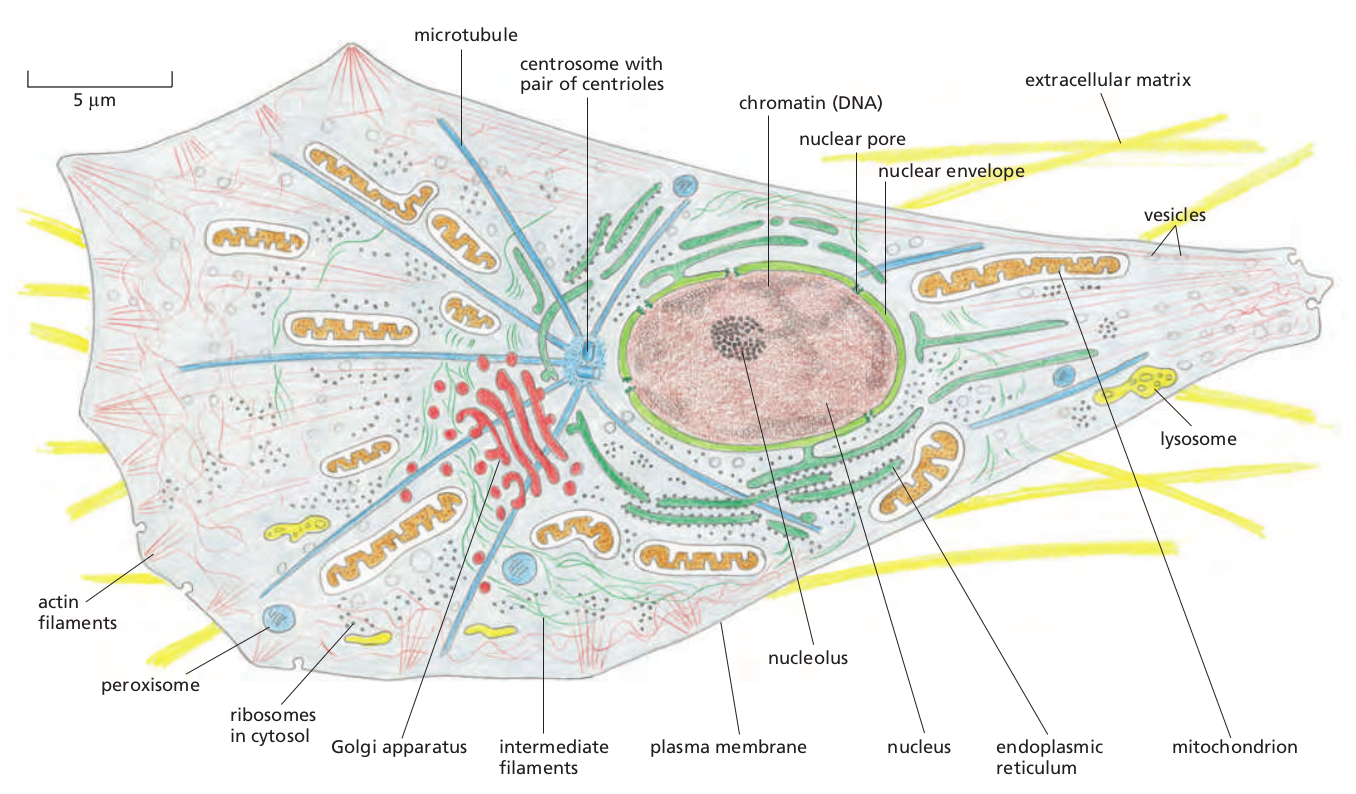
\includegraphics[width=0.5\textwidth]{celula_eucariota}}
  \subfloat[Dogma central de la biología molecular]{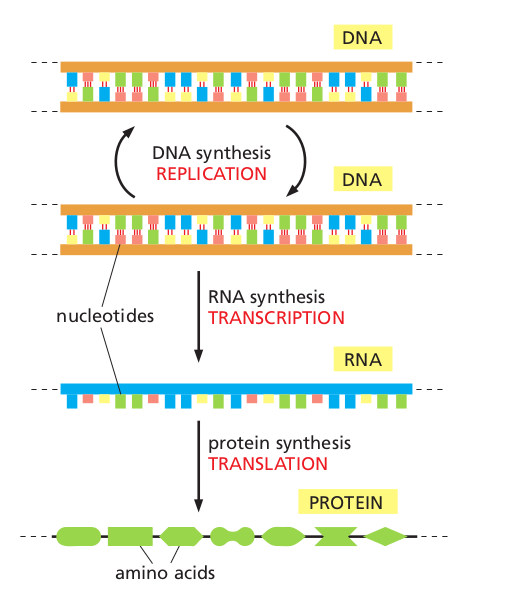
\includegraphics[width=0.5\textwidth]{adn3}}
\end{figure}

\end{frame}

\subsubsection*{Cambios transcripcionales}
\begin{frame}\frametitle{Cambios transcripcionales en respuesta a estrés abiótico en \textit{A. thaliana}} 
	\begin{columns}[T]
		\column{0.5\textwidth}
			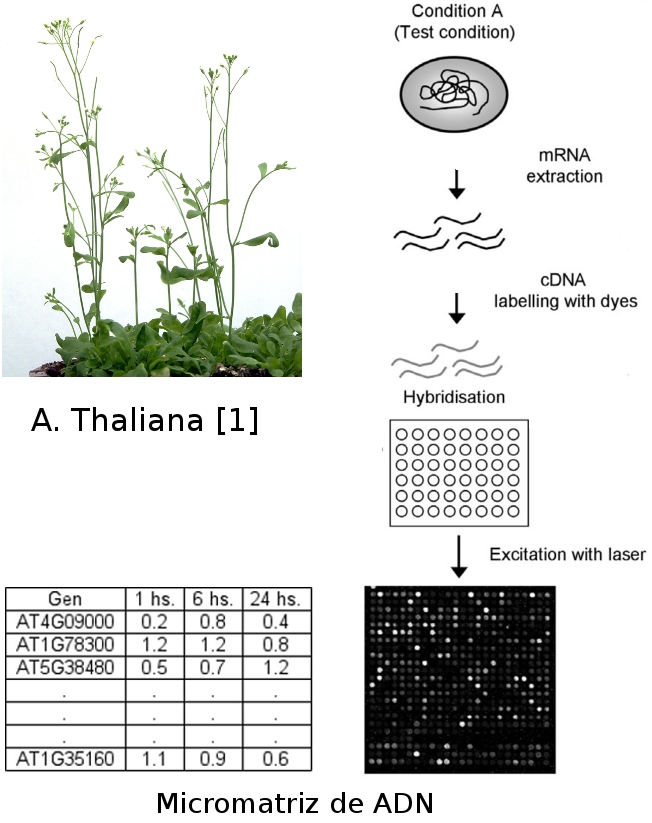
\includegraphics[width=1\textwidth]{micromatriz_y_arabidopsis}
		\column{0.5\textwidth}
			\bigskip
			\Large 
			Datos de estrés abiótico:
			\medskip
			\begin{itemize}
				\item 11 tratamientos
				\item $\approx 22000$ genes
				\item entre 4 y 8 mediciones temporales por gen y por tratamiento 
			\end{itemize}			
			\centering	
			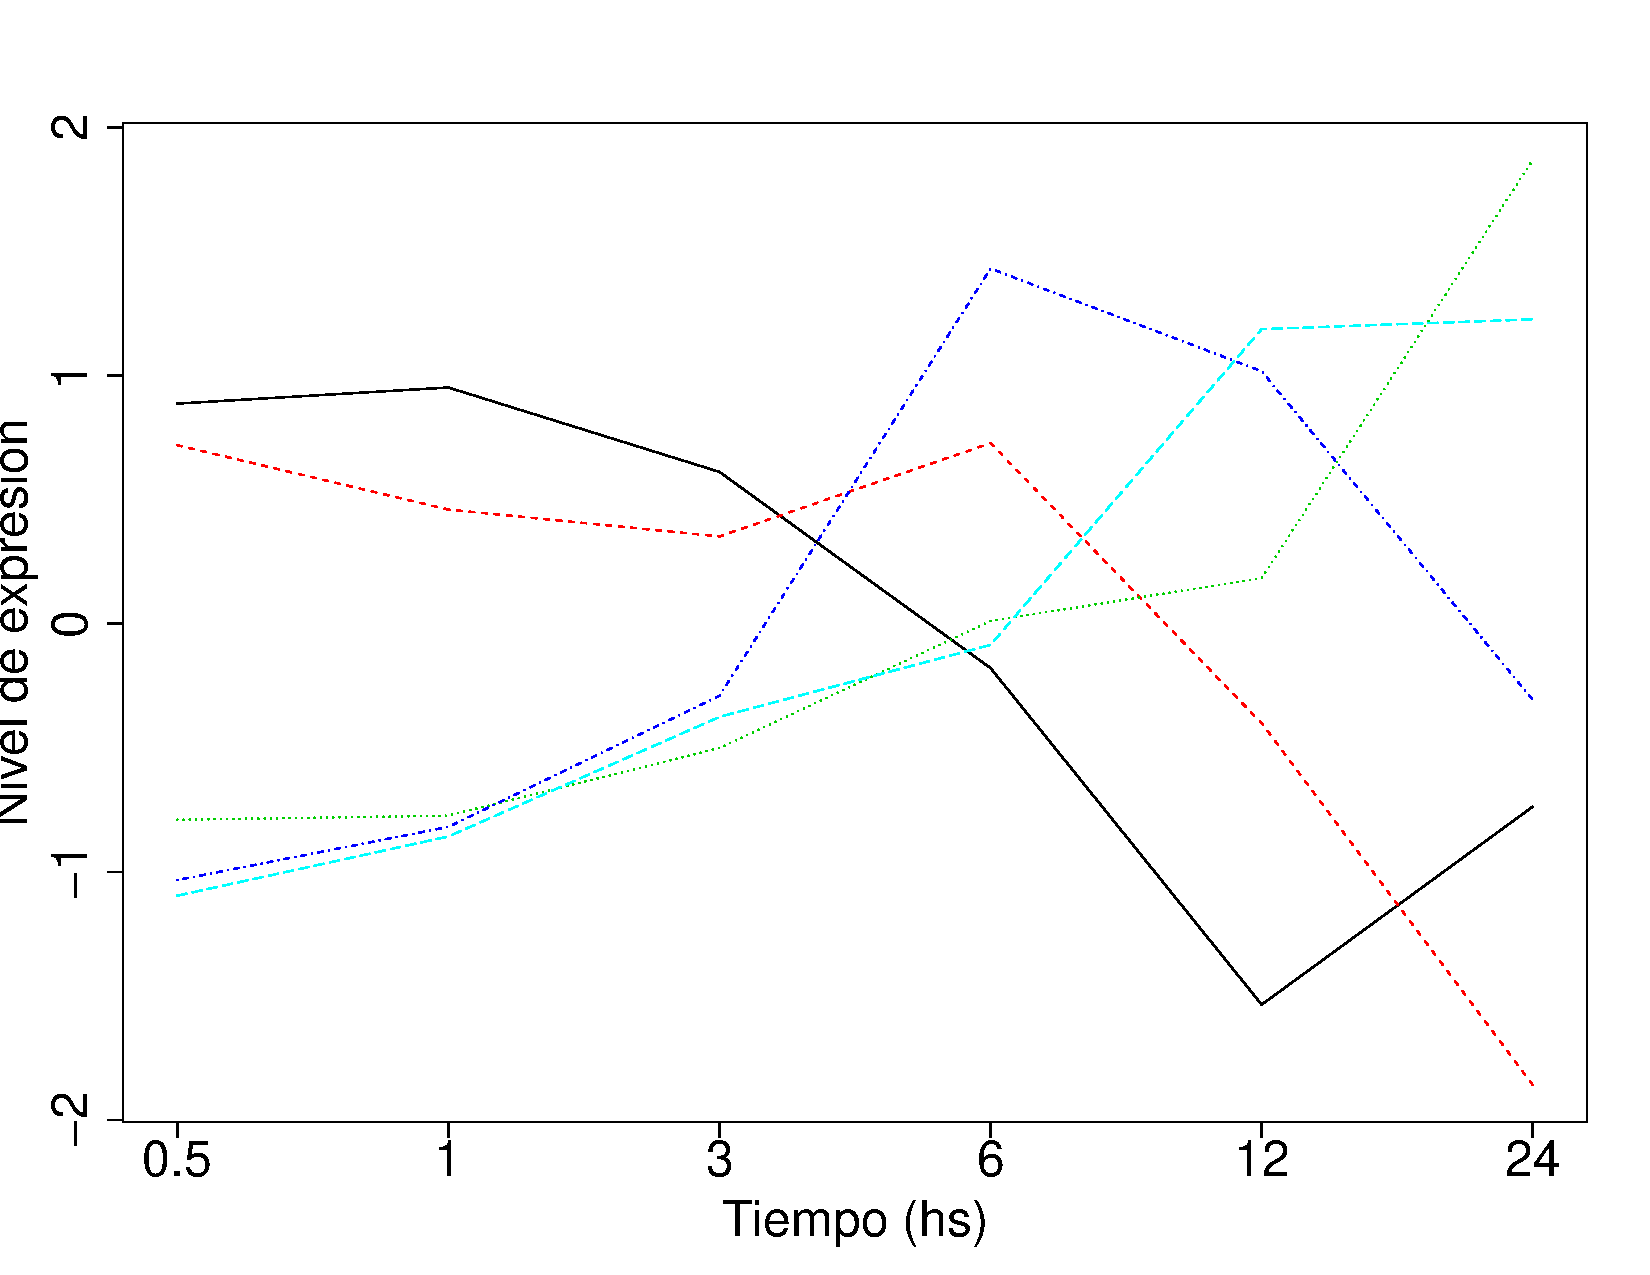
\includegraphics[width=0.9\textwidth]{perfiles_sin_agrupar.pdf}			
	\end{columns}
\end{frame}

\section{Análisis de relevamientos transcripcionales}

\subsection{Medidas de similaridad y distancia}
\begin{frame} \frametitle{Medidas de similaridad y distancia} 
\centering
Necesitamos definir que significa que dos datos sean ``similares''\bigskip
\begin{columns}[T]
\column{0.45\textwidth}
	Distancia euclidiana en espacio de alta dimensionalidad:\\
	\begin{equation}
		d_{euc}(\vec{x}, \vec{y}) = [\sum\limits_{i=1}^n (x_i-y_i)^2]^\frac{1}{2}
	\end{equation}
	\bigskip
	\centering
	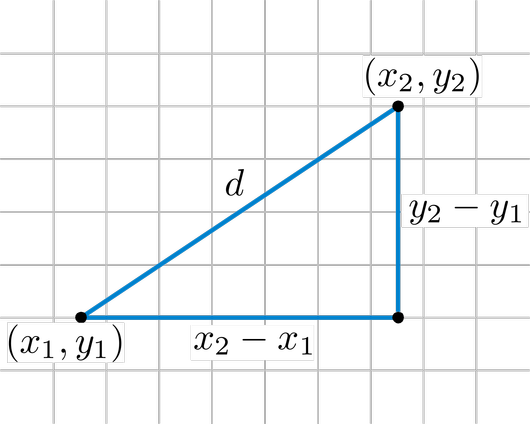
\includegraphics[width=0.7\textwidth]{distancia_euclidiana}

\column{0.55\textwidth}
	Distancia basada en el coeficiente de correlación de Pearson:\\
	\begin{equation}
		r(\vec{x}, \vec{y}) = \frac{\frac{1}{n-1}\sum\limits_{i=1}^n(x_i-\bar{x})(y_i-\bar{y})}{s_x s_y}
	\end{equation}
	\begin{equation}
		d_{ccp}(\vec{x}, \vec{y}) = 1-r(\vec{x}, \vec{y})
	\end{equation}
	\centering	
	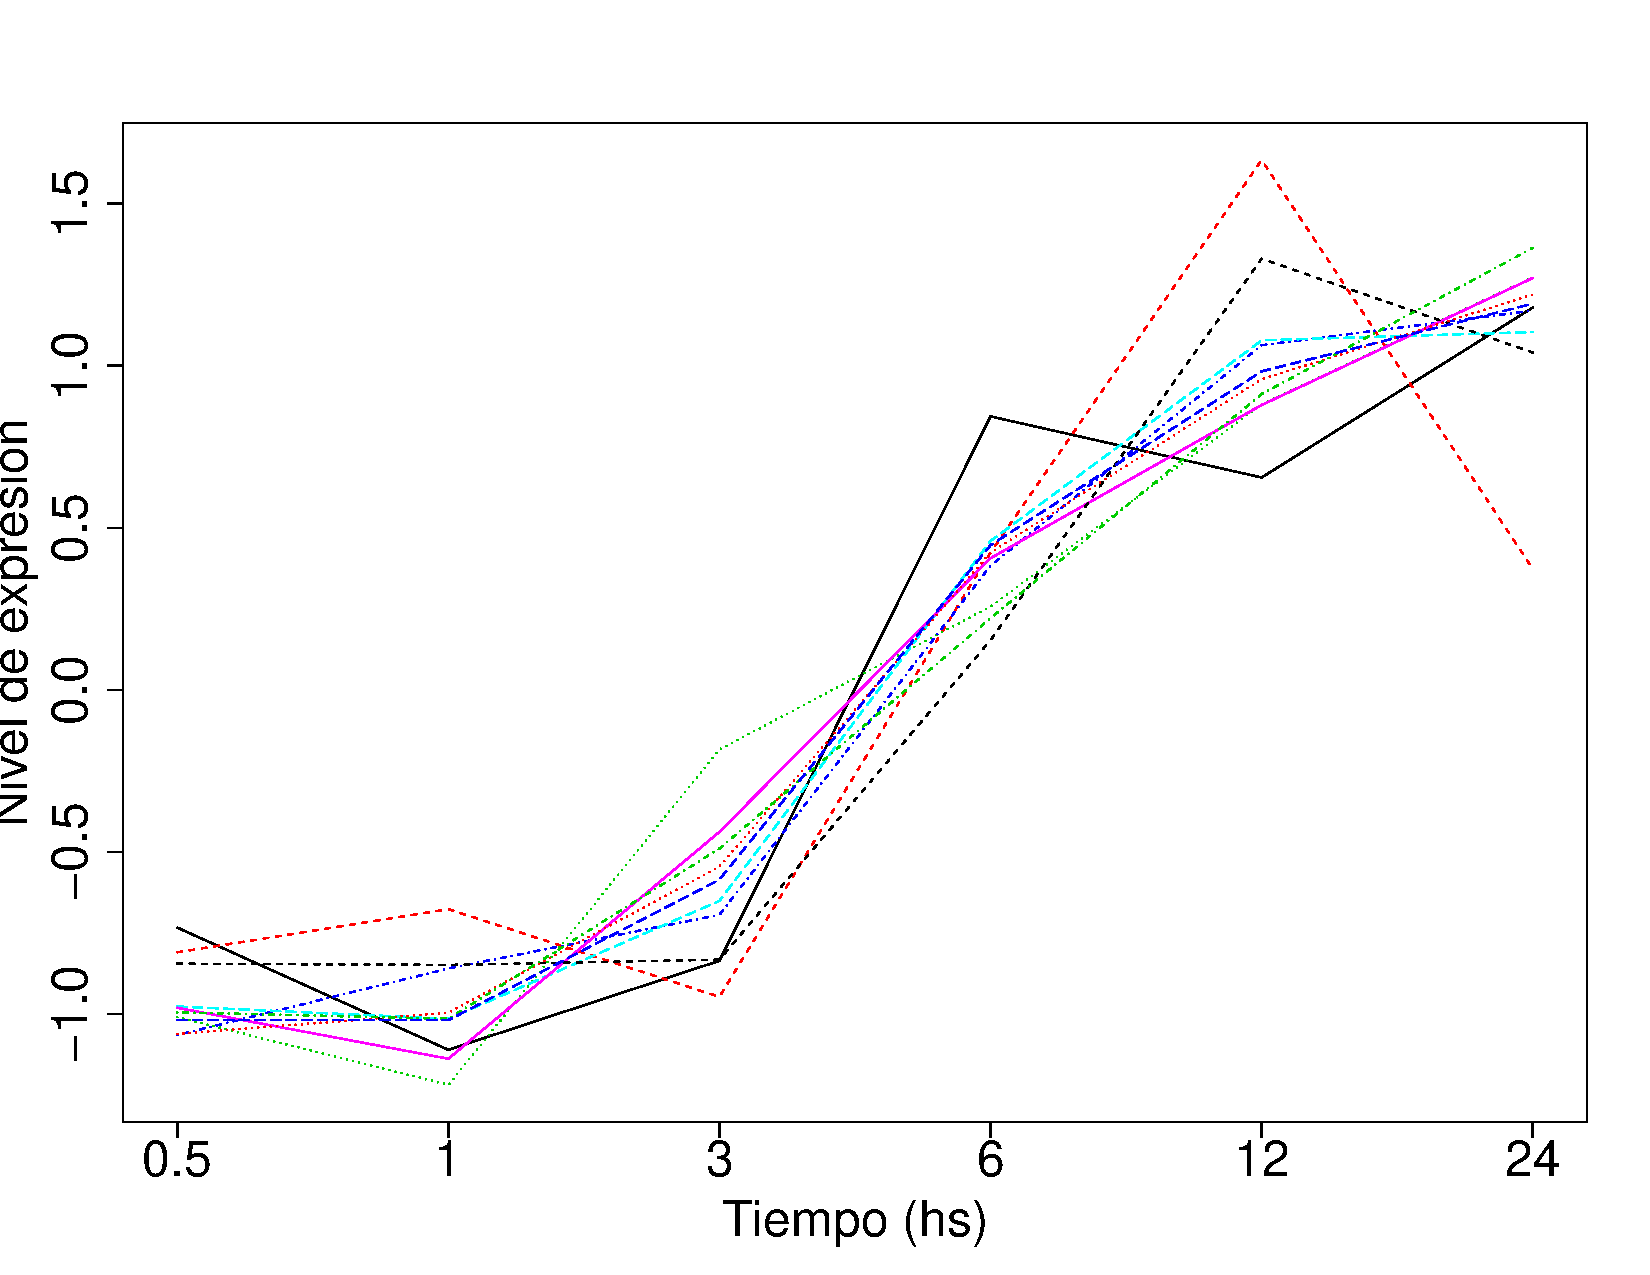
\includegraphics[width=0.7\textwidth]{perfiles_coregulados.pdf}
\end{columns}

\end{frame}

\subsection{Métodos de agrupamiento utilizados}
\begin{frame}\frametitle{Método de agrupamiento k-means} 
\begin{columns}[T]
\column{0.5\textwidth}
	\begin{itemize}
	\item Agrupamiento no jerárquico.
	\item Cada observación pertenece al grupo con la media más cercana.
	\item La cantidad k de grupos debe ser fijada a priori.
	\item Utiliza la distancia euclidiana.
	\end{itemize}
	Para datos estandarizados:
	\begin{equation}
		\tilde{x_i} = \frac{x_i-\bar{x}}{s_x}
	\end{equation}	
	la distancia euclidiana se relaciona con la correlación como:
	\begin{equation}
		d(\vec{x}, \vec{y}) = \sqrt{2(n-1)(1-r(\vec{x}, \vec{y}))}
	\end{equation}

\column{0.5\textwidth}
	\centering	
	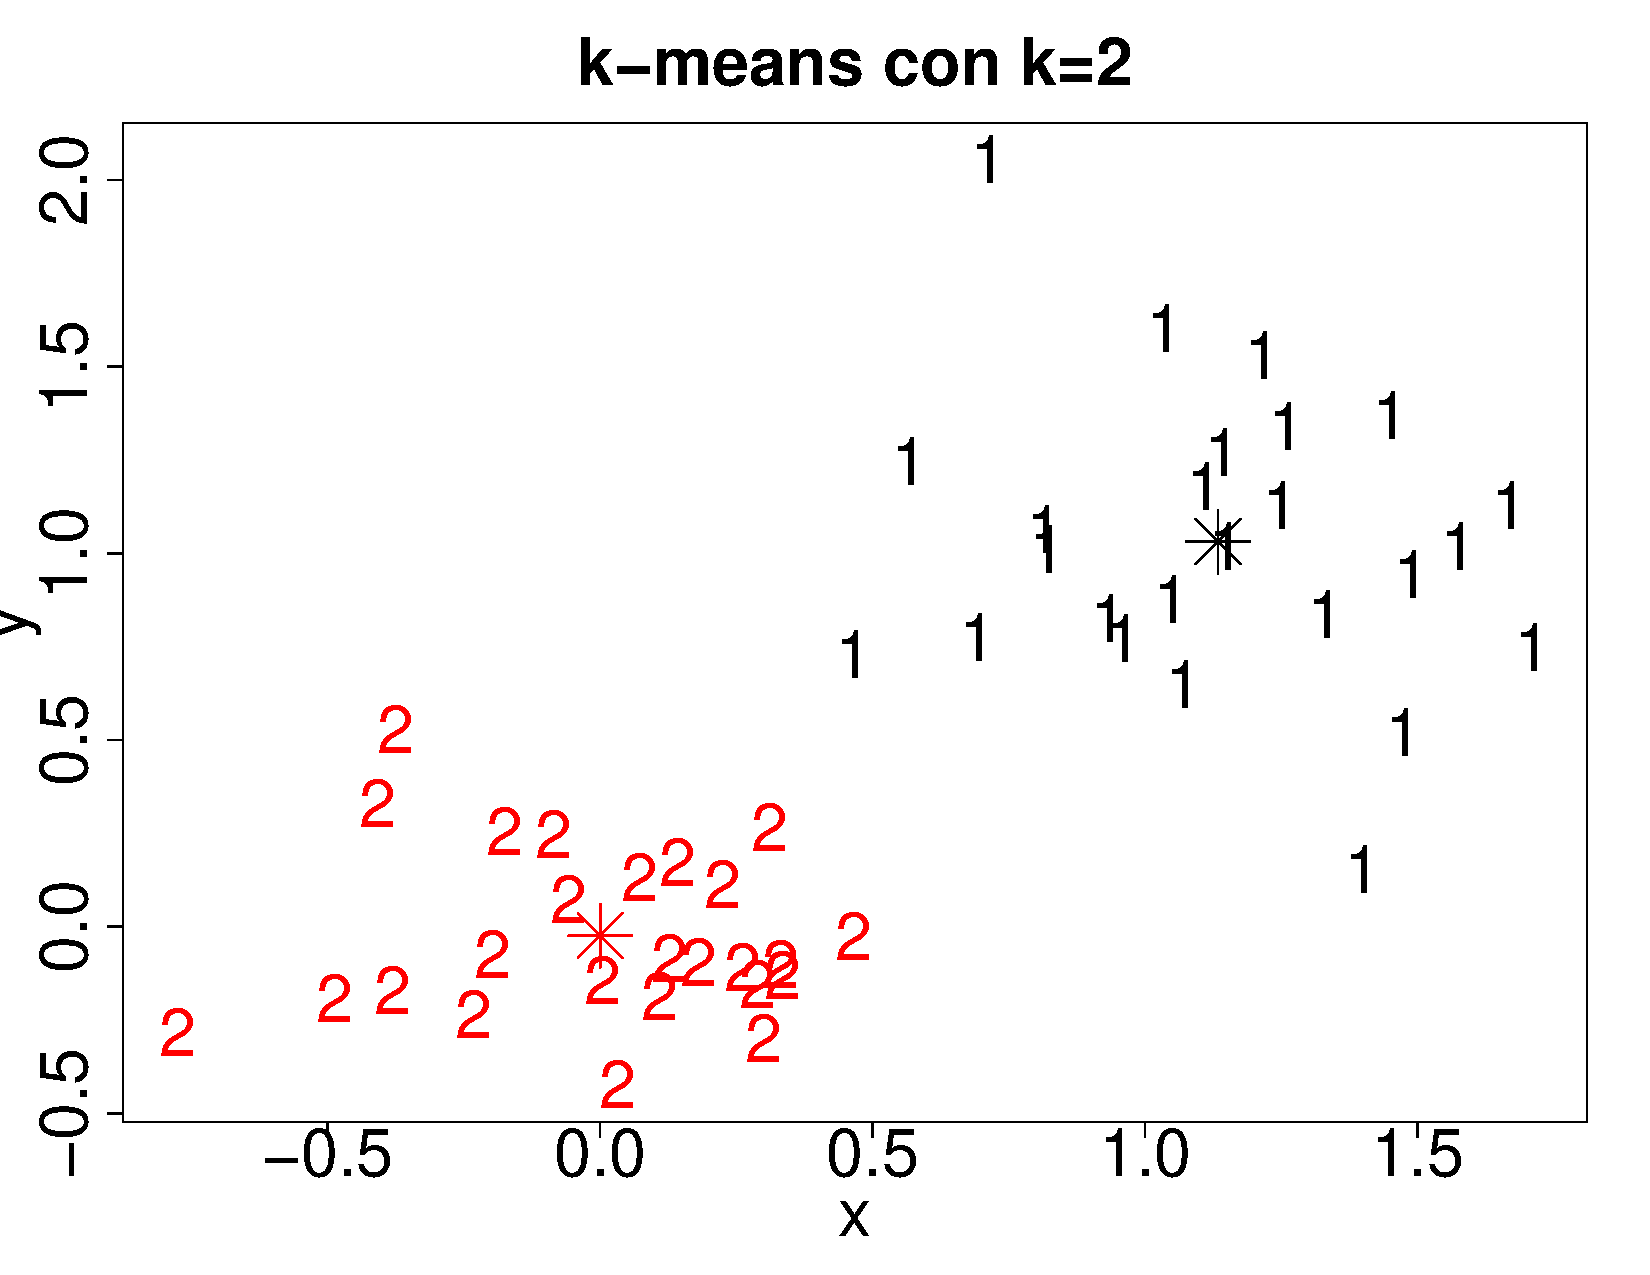
\includegraphics[width=0.8\textwidth]{ejemplo_kmeans_k2.pdf}
	
	\centering	
	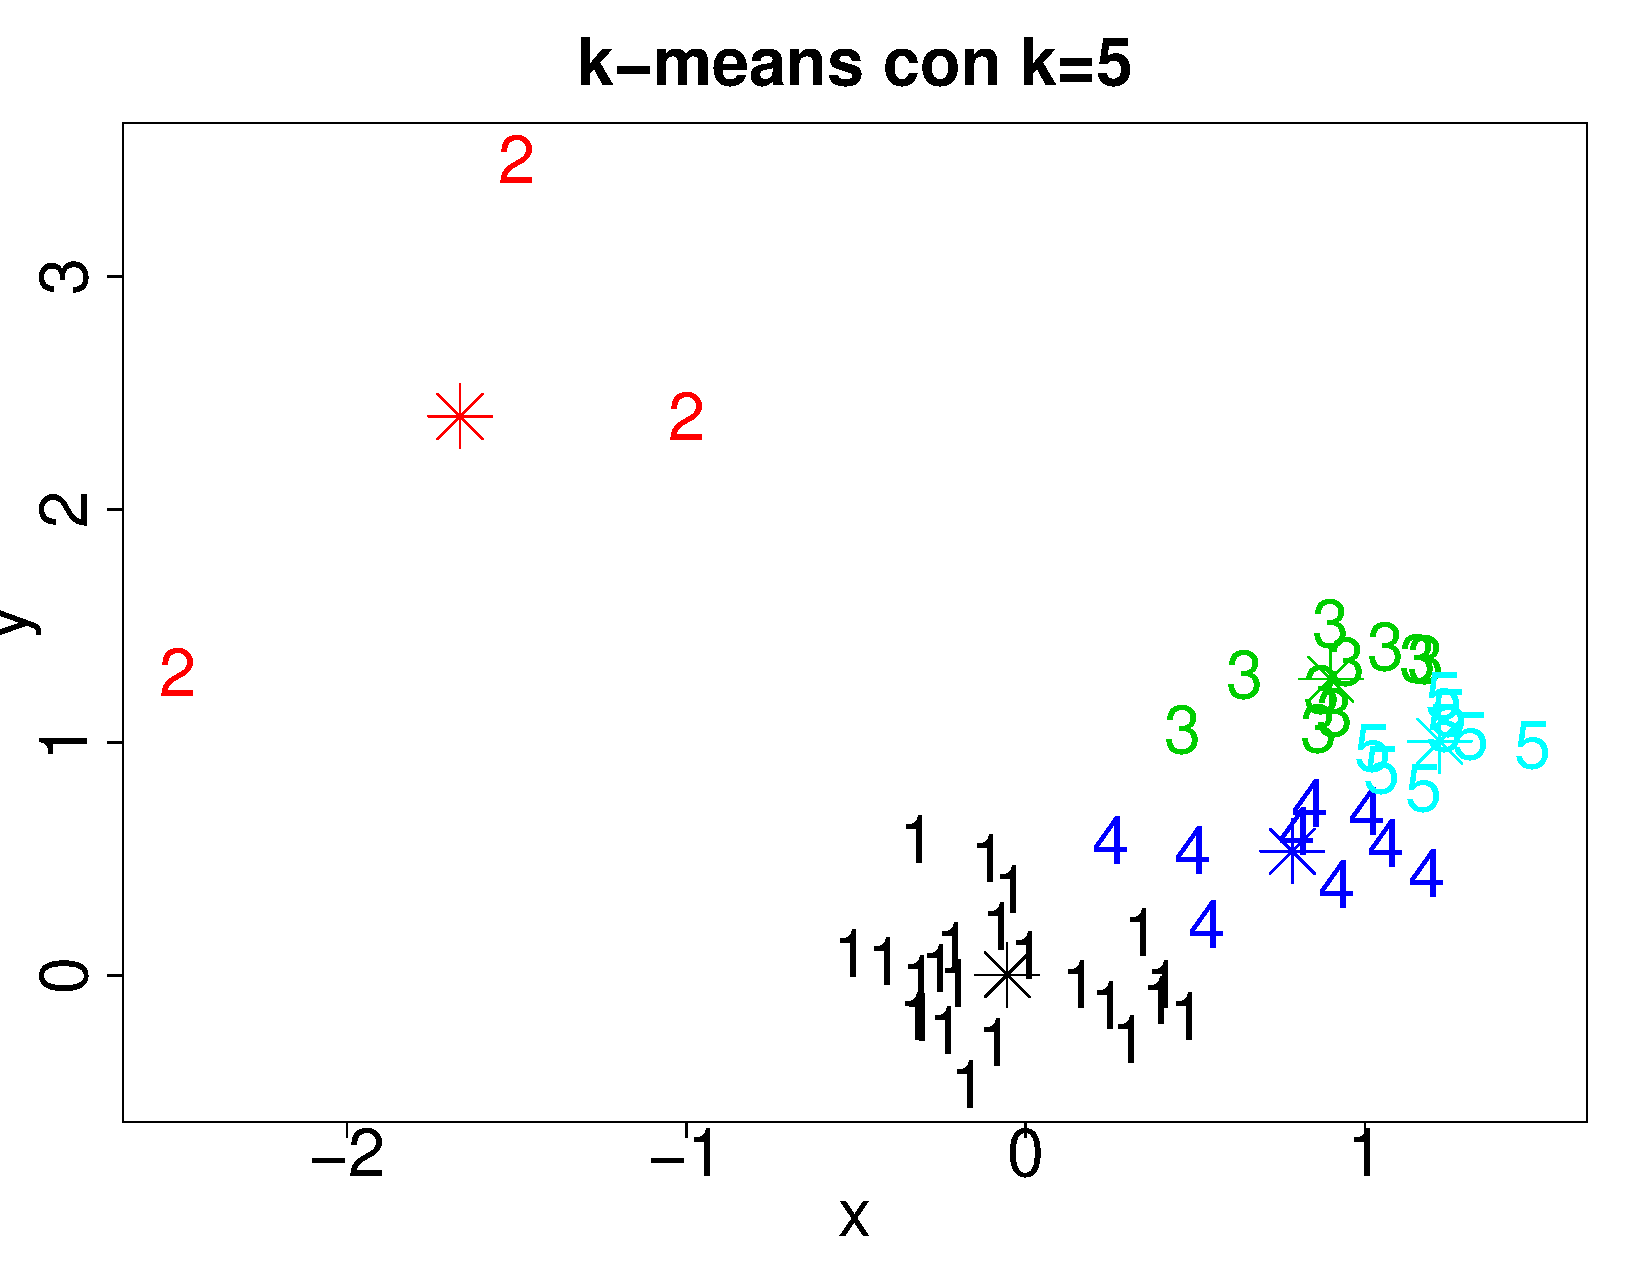
\includegraphics[width=0.8\textwidth]{ejemplo_kmeans_k5.pdf}	
\end{columns}
\end{frame}

\subsection{Métodos de agrupamiento utilizados}
\begin{frame}\frametitle{Método de agrupamiento corte de árbol dinámico} 
\centering
\begin{itemize}
\item Agrupamiento jerárquico.
\item Utiliza la distancia de correlación.
\item Se puede ``sintonizar'' la resolución del método. 
\item DS1 particiones gruesas, con pocos grupos bien definidos.
\item DS4 particiones finas, con muchos grupos más dispersos.
\end{itemize}
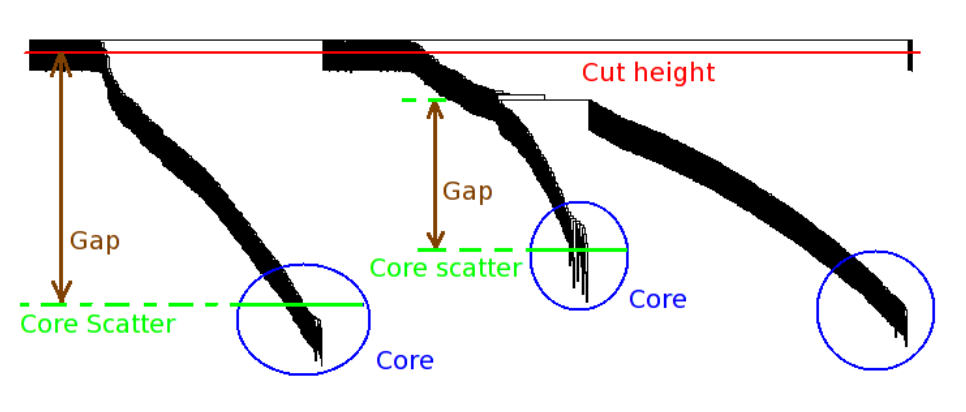
\includegraphics[height=0.55\textheight]{cut_tree_dynamic_ejemplo}	
\end{frame}

\subsection{Caracterización de particiones}
\begin{frame}\frametitle{Perfiles tratamiento ``Frío'' con k-means} 
\centering
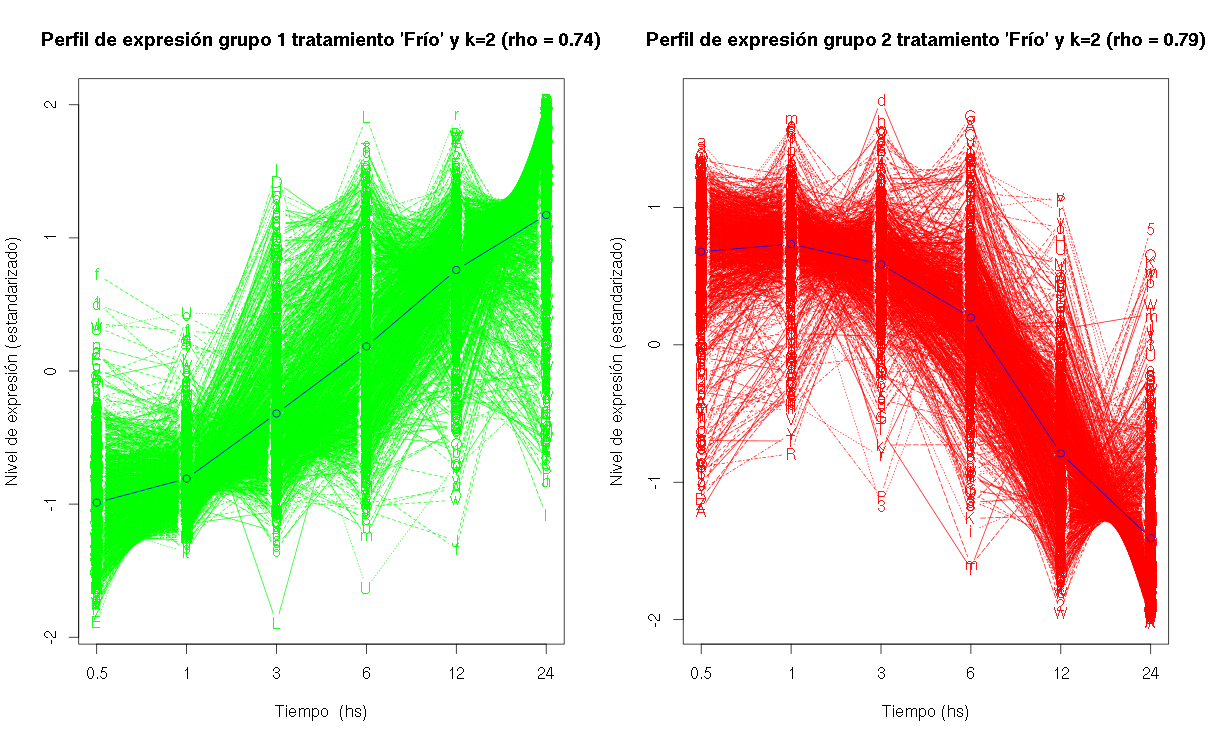
\includegraphics[width=1\textwidth]{perfiles_k_means}	
\end{frame}

\begin{frame}\frametitle{Perfiles tratamiento ``Frío'' con corte de árbol dinámico} 
\centering
A modo de ejemplo, los nueve perfiles más grandes de cada partición
\begin{columns}[T]
\column{0.5\textwidth}
	\centering
	DS1 (particiones más gruesas)
	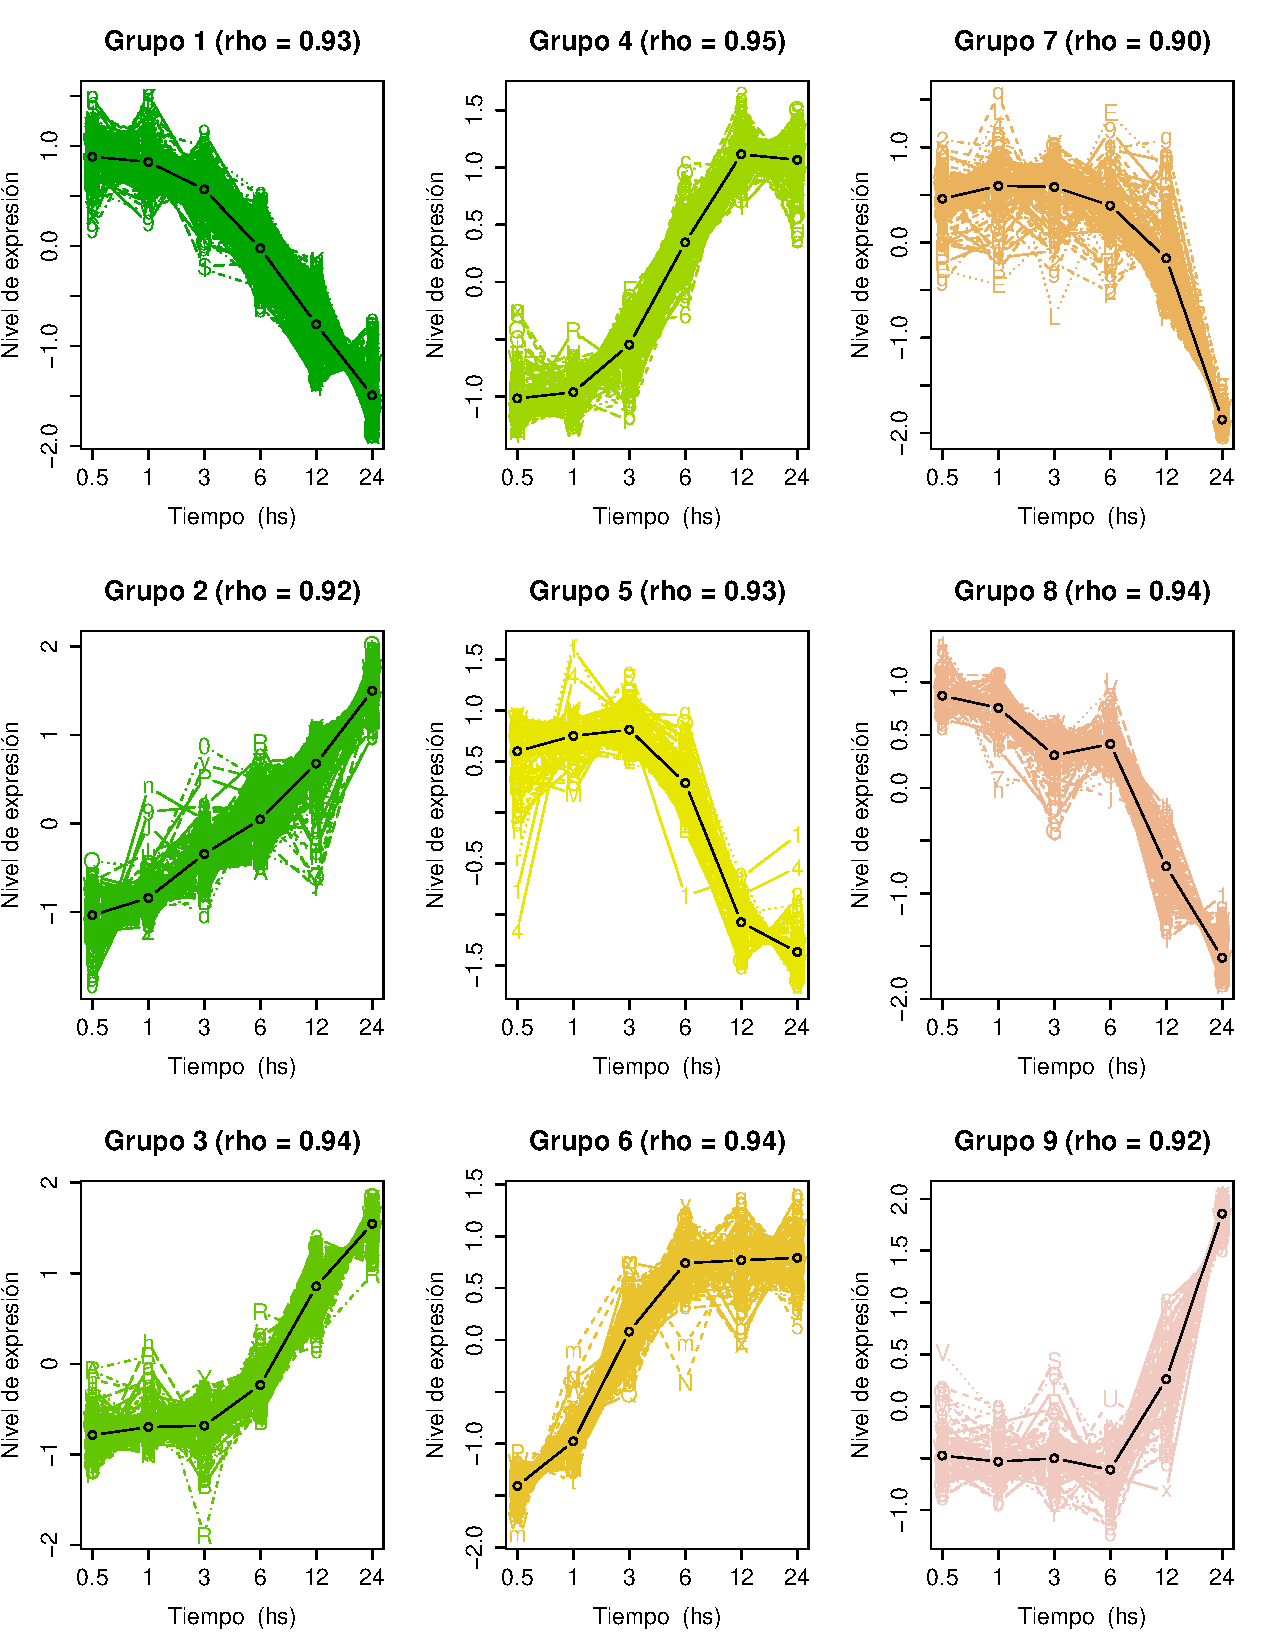
\includegraphics[width=0.9\textwidth]{perfiles_ds_1.pdf}	
\column{0.5\textwidth}
	\centering
	DS4 (particiones más finas)
	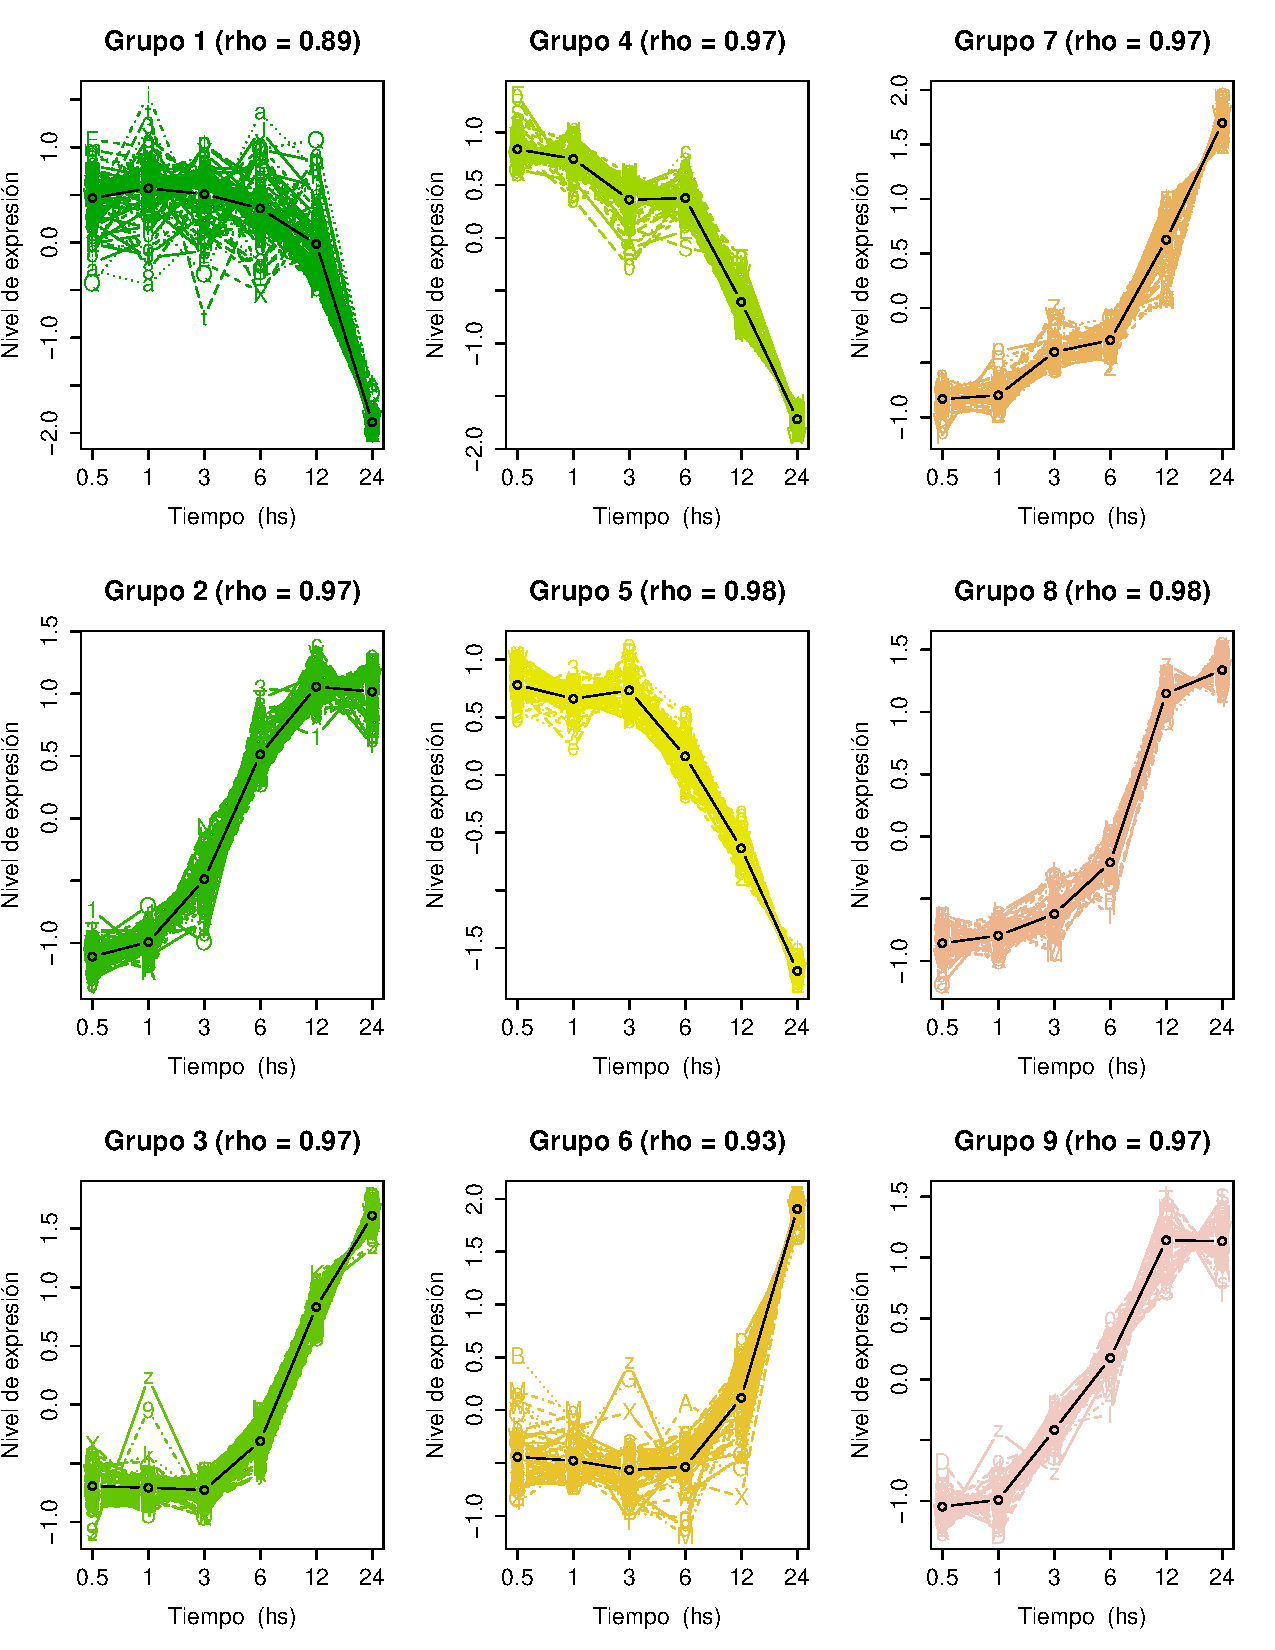
\includegraphics[width=0.9\textwidth]{perfiles_ds_4.pdf}	
\end{columns}
\end{frame}

\begin{frame}\frametitle{Caracterización de particiones corte de árbol dinámico} 
\centering
Correlación media por tamaño de grupo
\begin{columns}[T]
\column{0.5\textwidth}
	\centering
	DS1 (particiones más gruesas)
	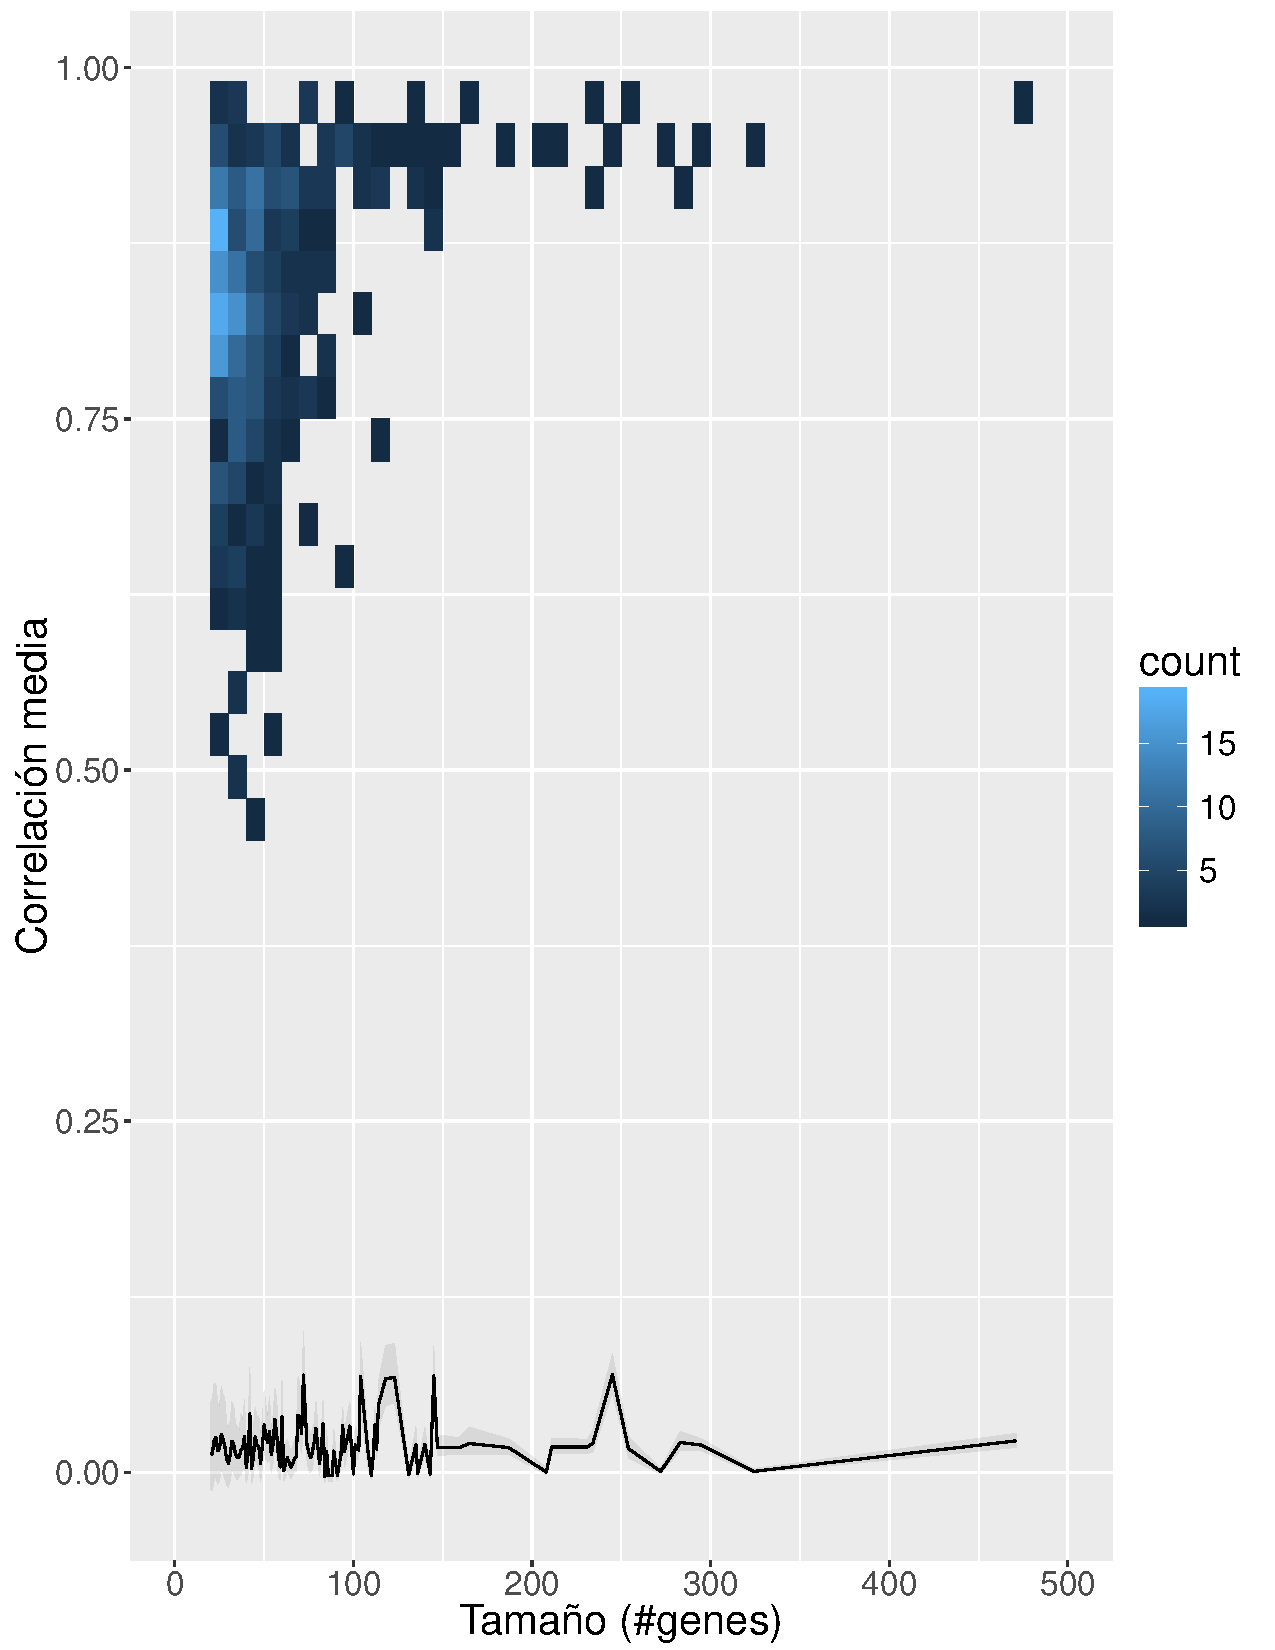
\includegraphics[width=0.9\textwidth]{correlacion_media_por_tamano_ds_1.pdf}	
\column{0.5\textwidth}
	\centering
	DS4 (particiones más finas)
	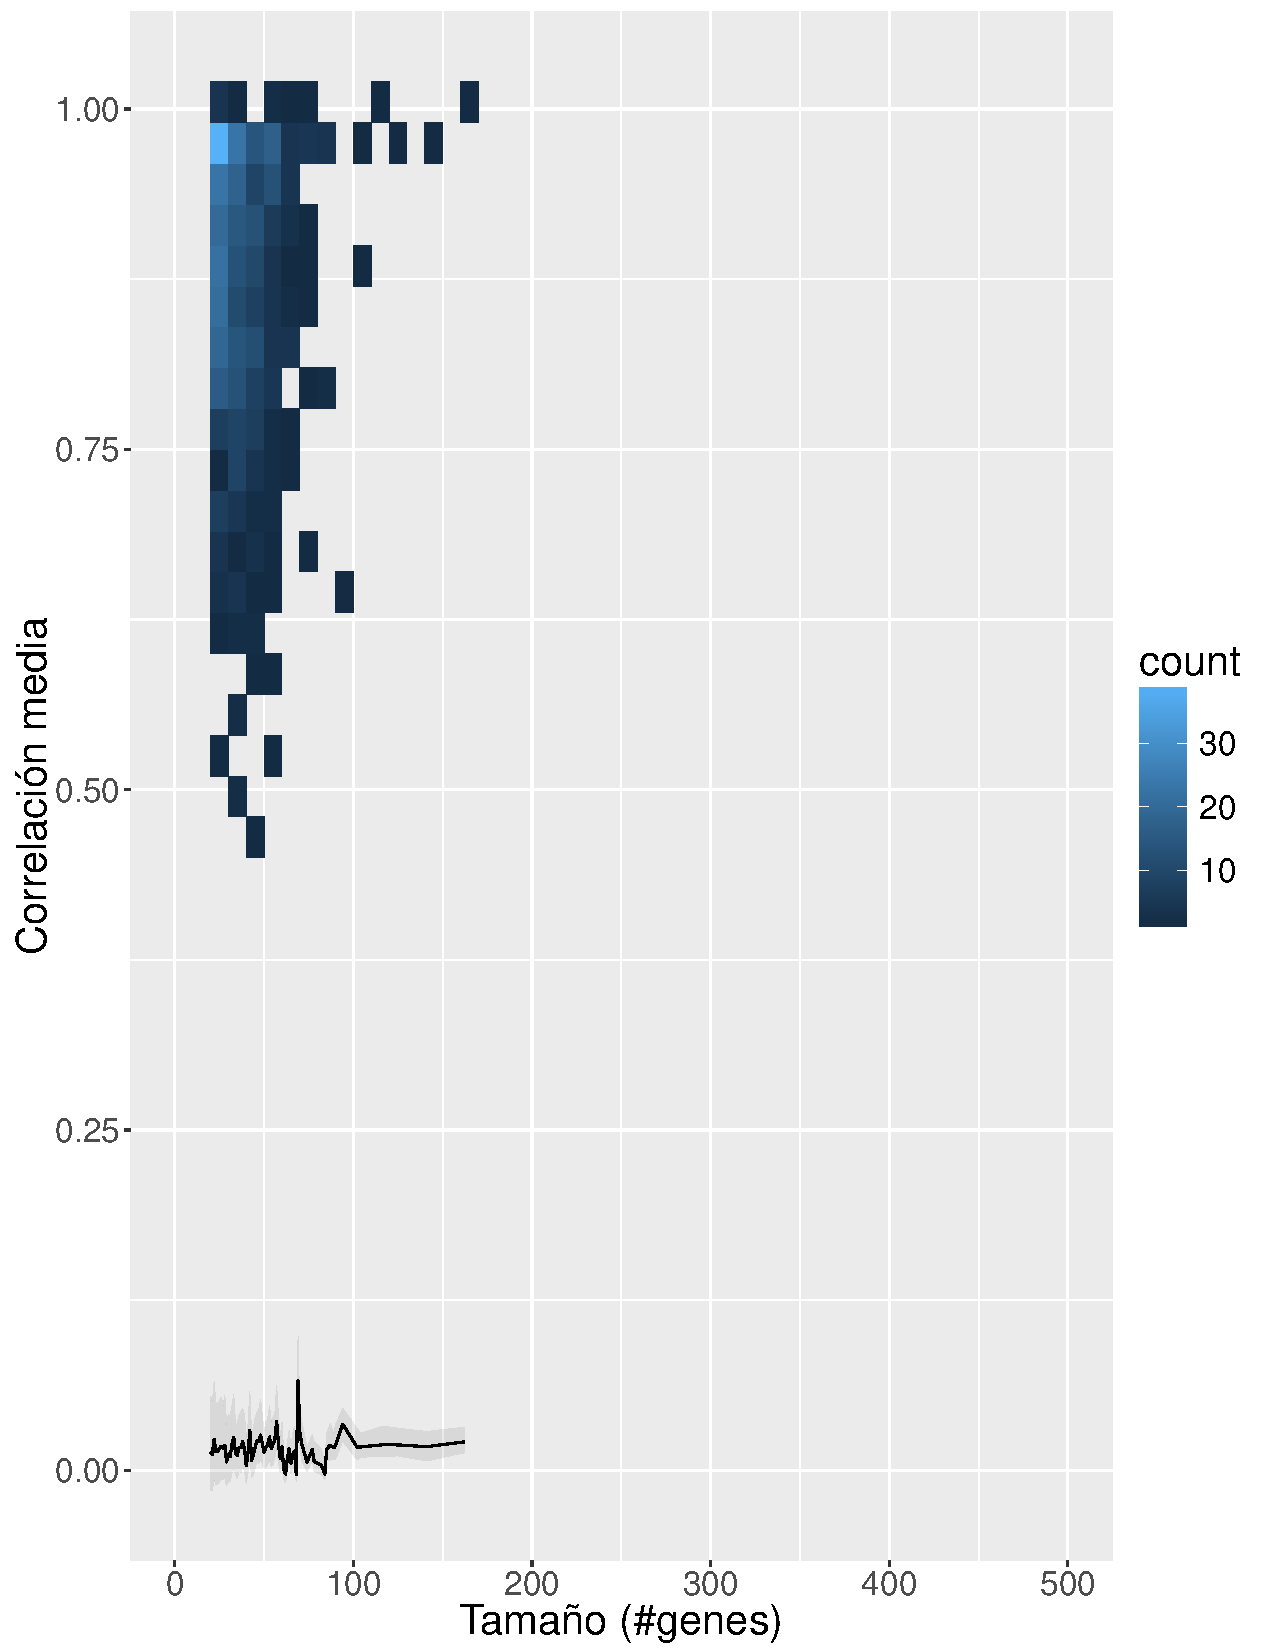
\includegraphics[width=0.9\textwidth]{correlacion_media_por_tamano_ds_4.pdf}	
\end{columns}
\end{frame}


\begin{frame}\frametitle{Caracterización de granularidad de las particiones halladas} 
\centering
Fracción de grupos en una partición más fina dentro de grupos de una partición más gruesa (tratamiento ``Frío'')
\begin{figure}
    \centering
	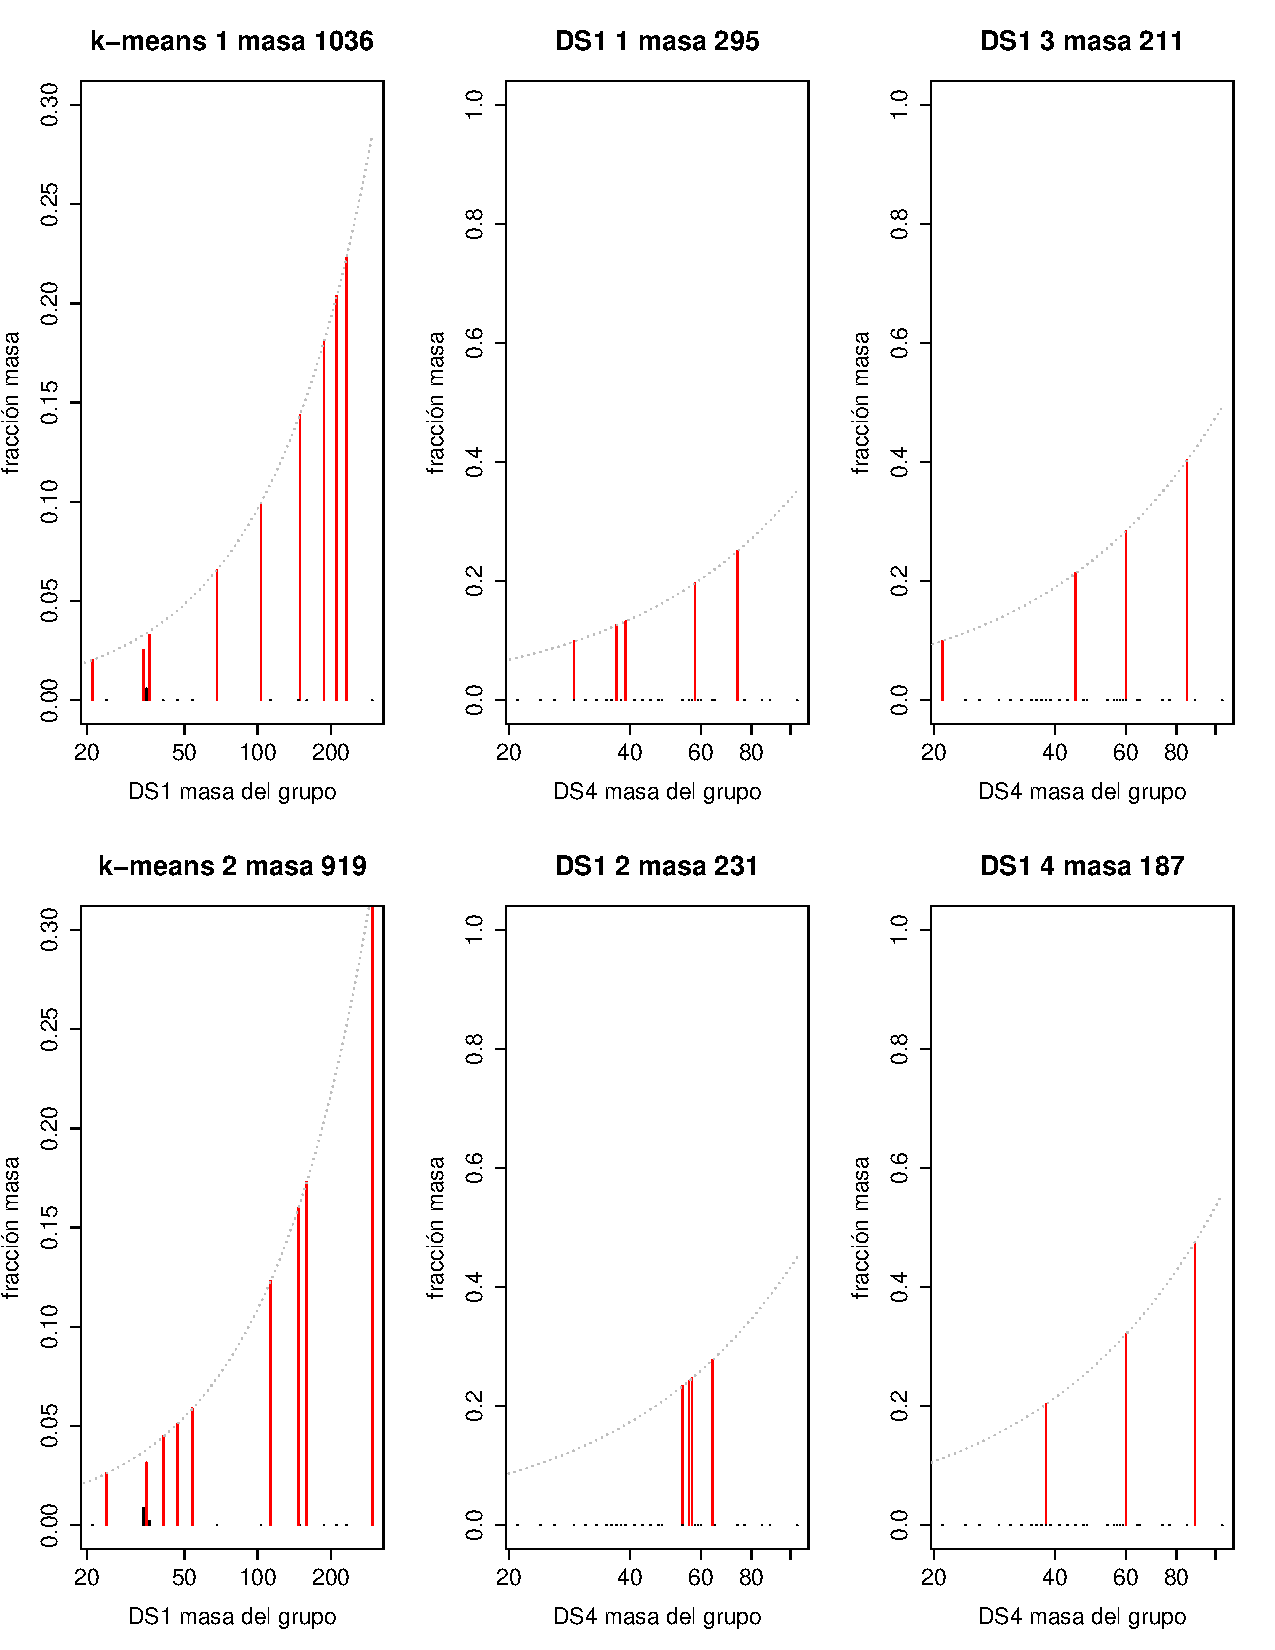
\includegraphics[height=1.6\textheight]{fraccion_de_km_en_ds1_en_ds4.pdf}	
\end{figure}
\end{frame}

\section{Congruencia biológica}

\subsection{Ontología génica (GO)}
\begin{frame}\frametitle{Ontología génica (GO)}
\begin{columns}[T]
	\column{0.5\textwidth}
	\begin{itemize}
		\item Provee un vocabulario controlado de términos.
		\item Permite comparar y clasificar entidades biológicas.
		\item Tres ontologías: procesos biológicos (BP), componentes celulares (CC) y funciones moleculares (MF).
		\item Estructura de grafo acíclico dirigido (DAG).
		\item Cada nodo representa un témino que describe alguna función.
		\item Los nodos se unen entre si por medio de relaciones ``es un'' o ``es parte de''.
		\item Un gen descrito por un término está ``anotado'' en ese término.
	\end{itemize}
	\column{0.5\textwidth}
	\centering
	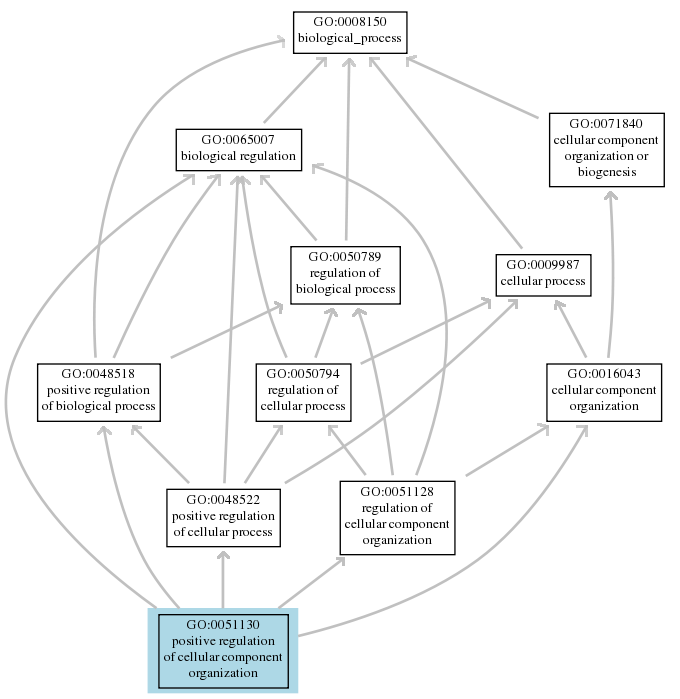
\includegraphics[width=1.1\textwidth]{ejemplo_de_go}	
\end{columns}
\end{frame}

\subsection{Cuantificando la congruencia biológica}
\begin{frame}\frametitle{Observables} 
\centering
Buscamos cuantificar la congruencia biológica de las particiones halladas
\bigskip
\begin{columns}[T]
	\column{0.5\textwidth}
	Densidad de interacción:\\
	\bigskip
	\begin{equation}
		ID(GO_j) = \frac{NE(GO_j)}{N(GO_j)}
	\end{equation}
	\bigskip
	Con $NE(GO_j)$ la cantidad de pares de genes anotados en $GO_j$ que se encuentran juntos en un mismo grupo 	transcripcional $C_x$ y $N(GO_j)$ la cantidad de pares de genes anotados en $GO_j$.
	\column{0.5\textwidth}
	Indice de homogeneidad biológica:\\
	\bigskip
	\begin{equation}
		BHI_j = \frac{1}{n_j(n_j-1)}\sum\limits_{x\neq y\in D_j}I(C(x)=C(y))
	\end{equation}
	\bigskip	
	Con $n_j$ la cantidad de genes anotados en el grupo $D_j$.\\
	La función indicadora $I(C(x)=C(y))$ que toma el valor $1$ si hay al menos una clase en donde ambos genes estén anotados, y $0$ en caso contrario.
\end{columns}
\end{frame}

\begin{frame}\frametitle{Densidad de interacción} 
\begin{columns}[T]
	\column{0.3\textwidth}
	\Fontvi
	\begin{enumerate}
	\item Términos mas específicos presentan mayor ID.
	\item Agrupamientos hasta 100 genes correlacionan con la información biológica embebida en la ontología.
	\item Las estructuras en KEGG presentan mayor congruencia con las ontologías, seguidas por AI1 y expresión.
	\item $ds1$ presenta mayor congruencia biológica que $ds4$. Indicio acerca de la escala de granularidad apropiada.
	\end{enumerate}
	\column{0.7\textwidth}
	\begin{figure}
	    	\centering
		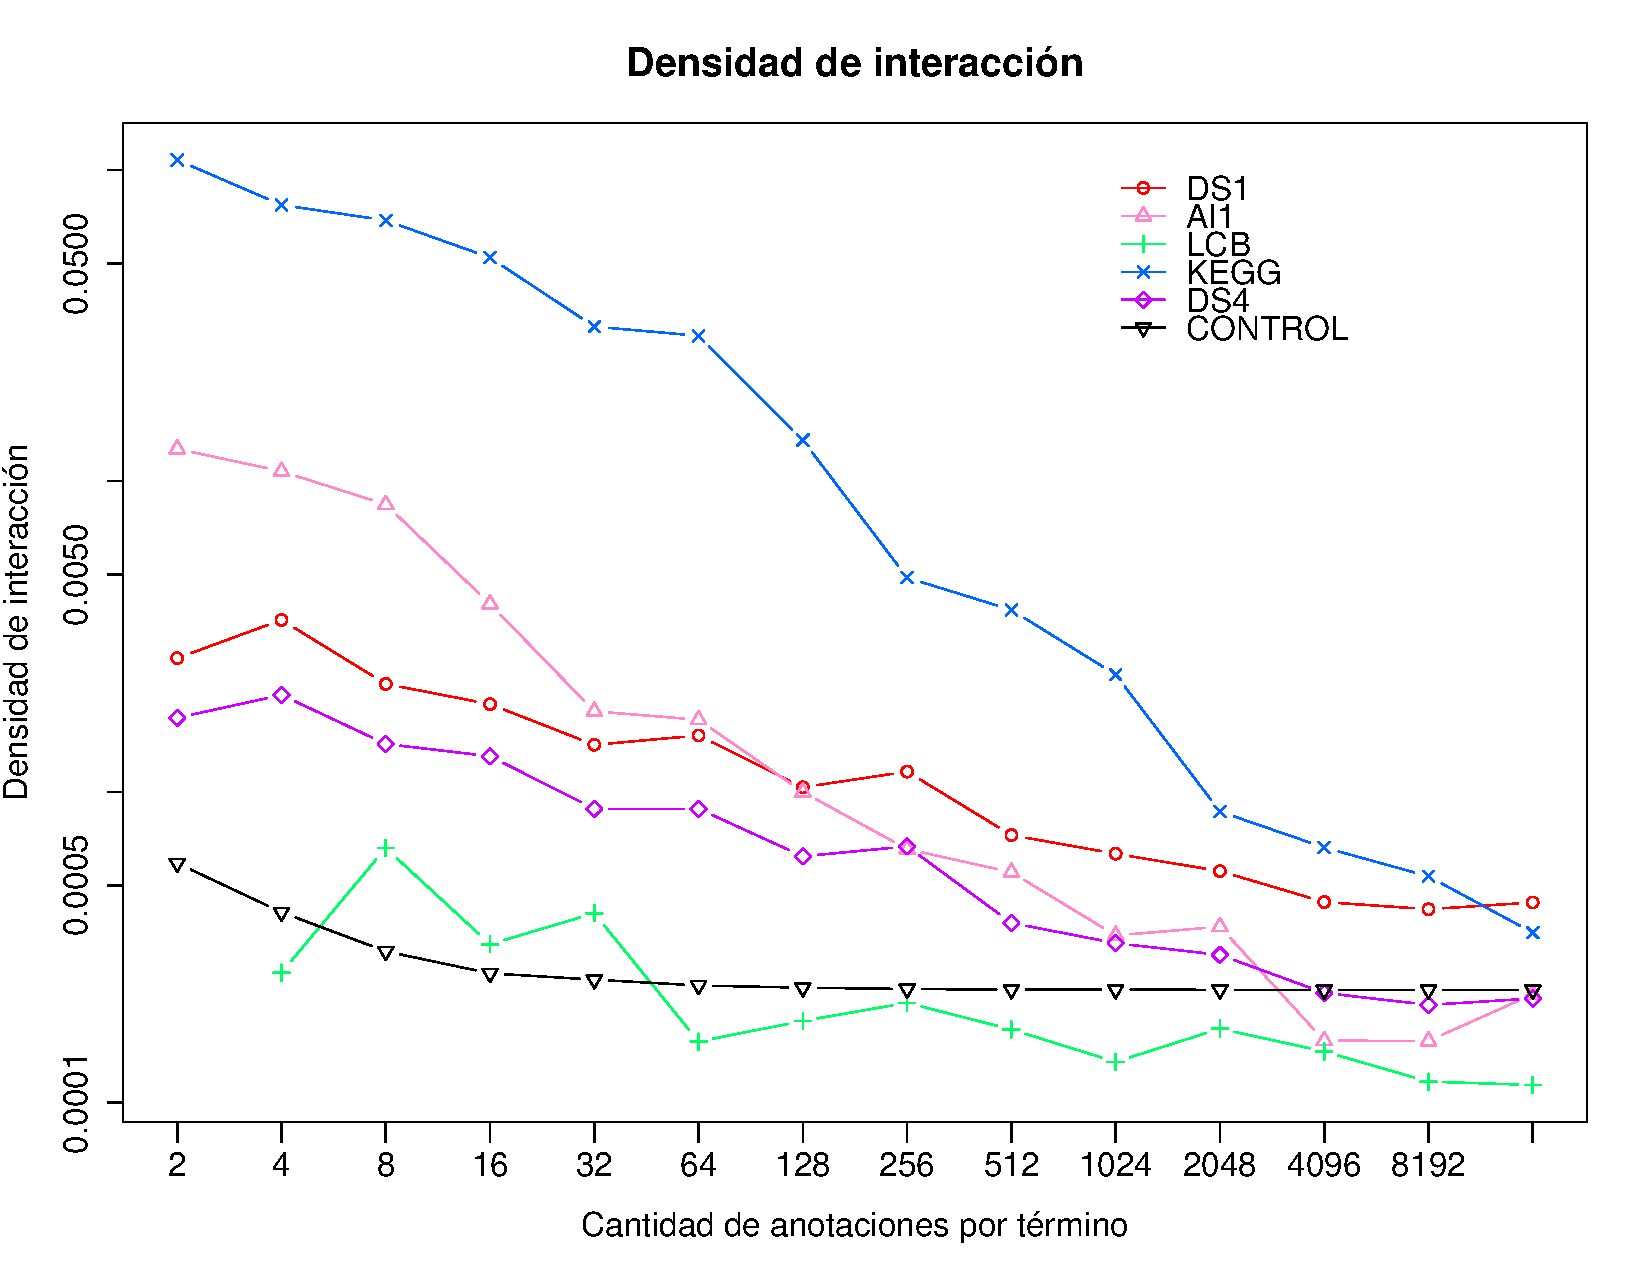
\includegraphics[width=1\textwidth]{interacting_densities_bpb.pdf}
	\end{figure}
\end{columns}
\end{frame}

\begin{frame}\frametitle{Indice de homogeneidad biológica} 
\begin{figure}
    	\centering
	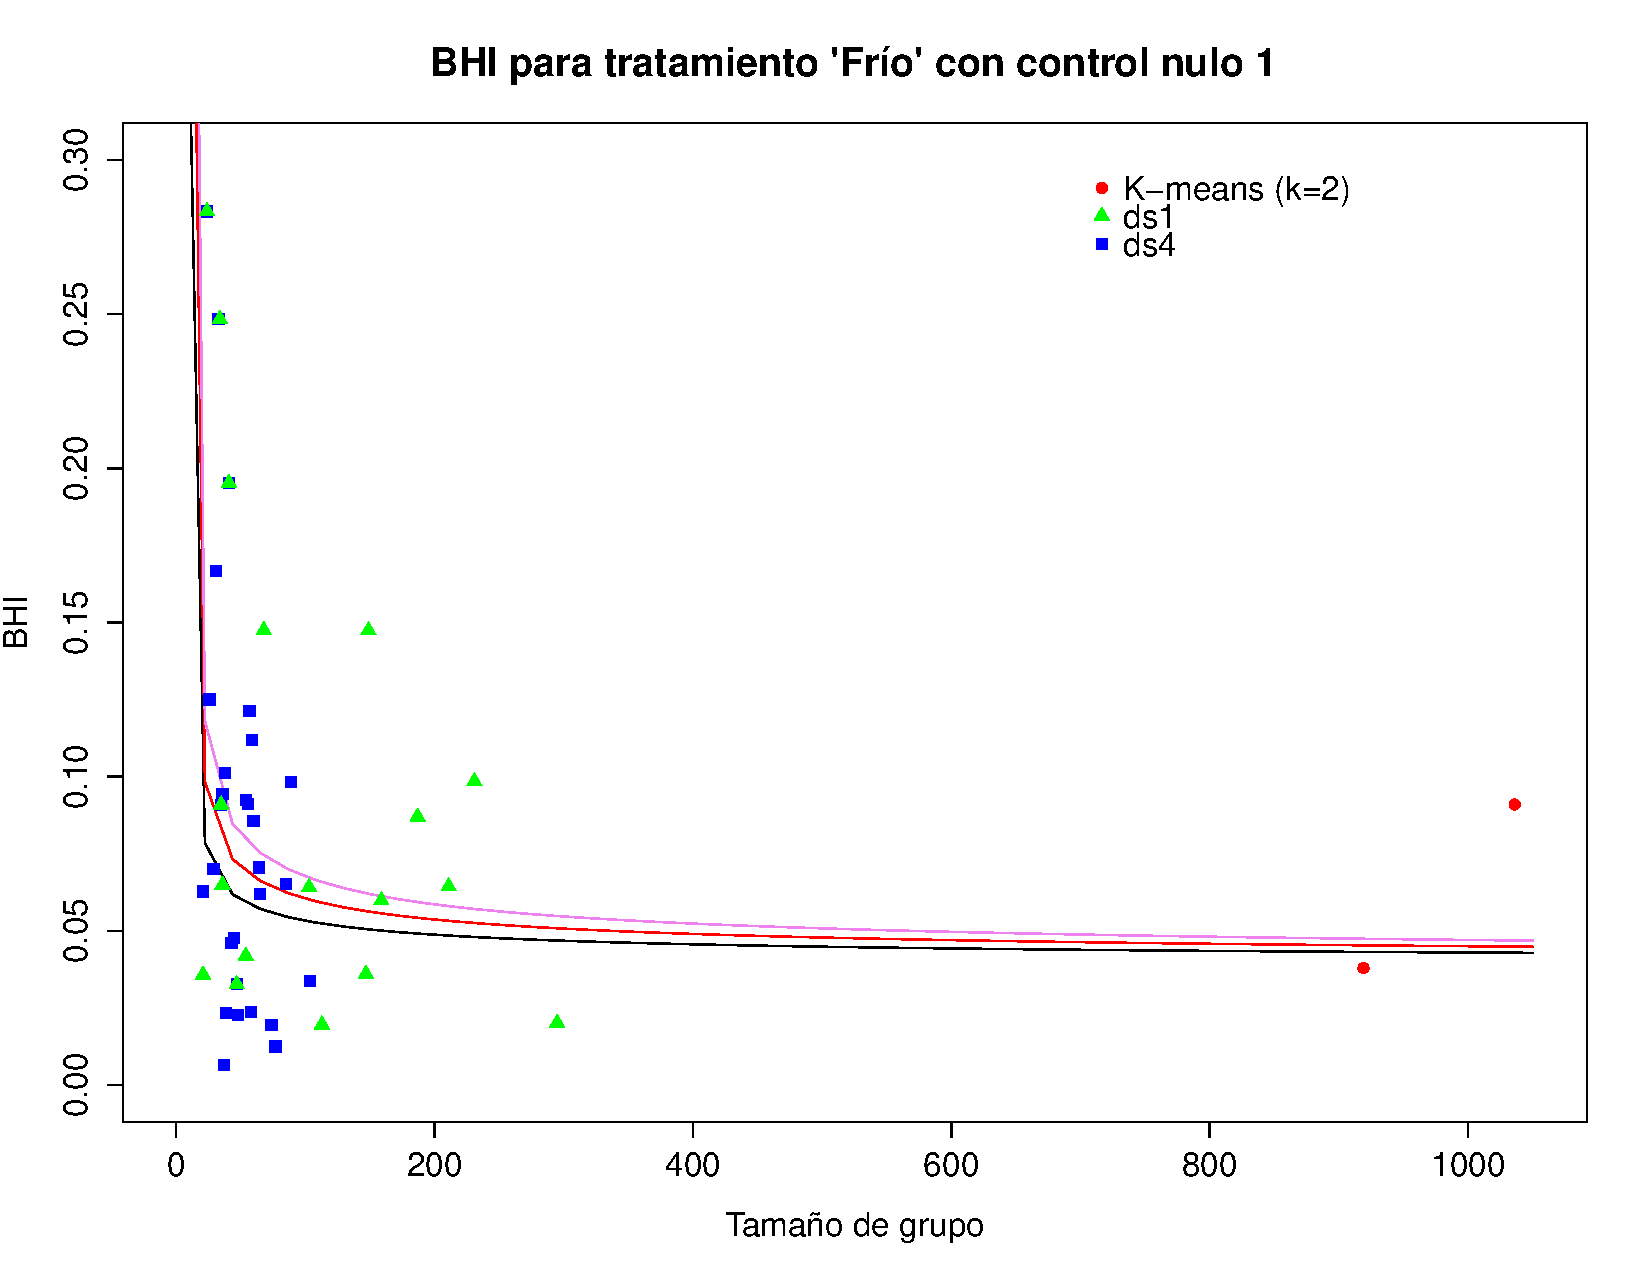
\includegraphics[width=0.8\textwidth]{bhi_km_ds1_ds4_control1.pdf}
\end{figure}
\centering
Particiones altamente coherentes pero de baja calidad de BHI.
\end{frame}

\section{Coherencia entre métricas}

\subsection{Métrica en GO}
\begin{frame}\frametitle{Similaridad entre genes en GO}
Definimos la similaridad entre genes en el espacio GO como:
\begin{equation}
	Sim_{rcmax}(GO(g_1), GO(g_2)) = \max\{\frac{1}{N}\sum\limits_{i}\max\limits_{1\leq j \leq M}S_{ij}, \frac{1}{M}\sum\limits_{j}\max\limits_{1\leq i \leq N}S_{ij}\}
\end{equation}
\bigskip
Donde:
\begin{equation}
	S(g_1, g_2)_{ij} = Sim_{res}(GO(g_1^i), GO(g_2^j)), \forall i \in \{1,...,N\} y \forall j \in \{1,...,M\}
\end{equation}
con:
\begin{equation}
	Sim_{res}(c_i, c_j) = \max\limits_{c \in S(c_i, c_j)}(-log_2[P(c)]) = IC(MICA[c_i, c_j])
\end{equation}
la similaridad entre términos.
\end{frame}

\subsection{KTA global}
\begin{frame}\frametitle{KTA global} 
La noción de similaridad de a pares en cada espacio esta dada en términos de una función $k$ llamada kernel tal que
\begin{equation}
	K = K_{ij} = k(x_i, x_j)
\end{equation}
\bigskip
El KTA de un kernel $k_1$ con respecto a un kernel $k_2$ del conjunto $C$ cuantifica la similaridad entre dos espacios y se define como:
\begin{equation}
	\hat{A}(C, k_1, k_2) = \frac{\langle K_1, K_2 \rangle _F}{\sqrt{\langle K_1, K_1 \rangle _F \langle K_2, K_2 \rangle _F}}
\end{equation}
con $\langle K_1, K_1 \rangle _F = \sum_{i,j=1}^m K1(x_i, x_j)K2(x_i, x_j)$ es el producto interno de Frobenius.\\
\end{frame}

\begin{frame}\frametitle{KTA global} 
\centering
KTA global entre expresión y ontología BP con control nulo
\begin{figure}
    	\centering
	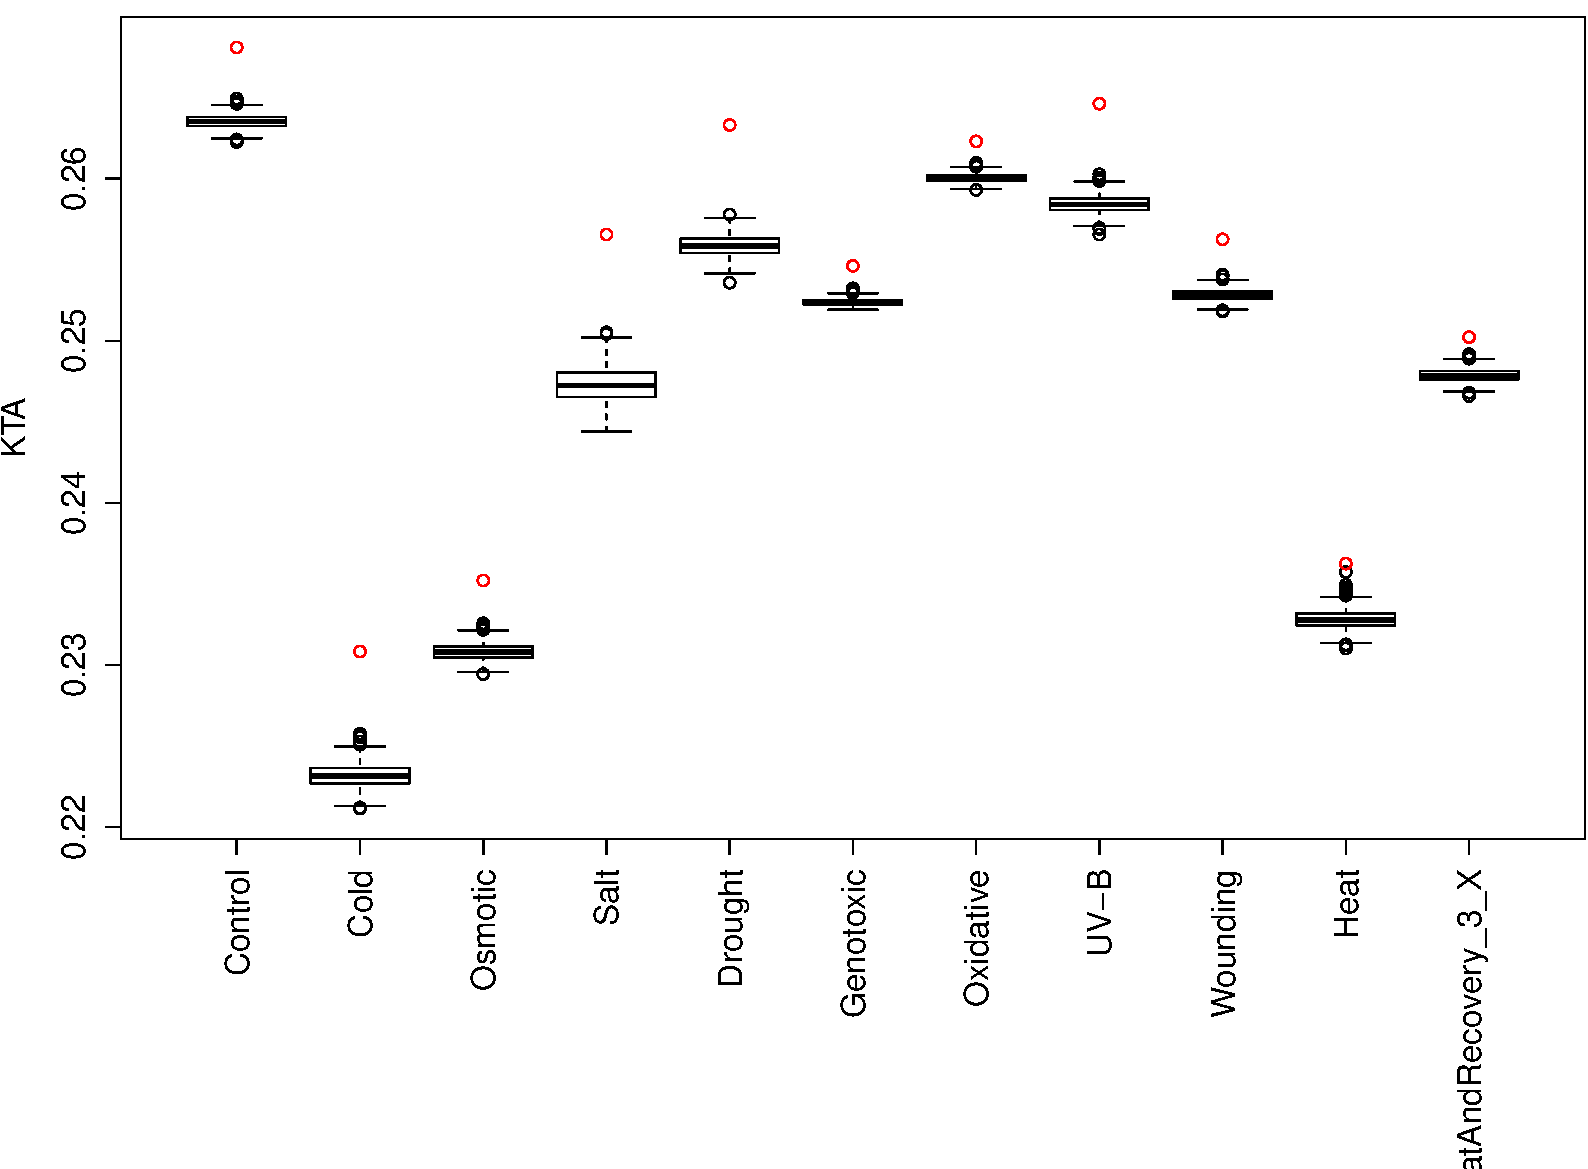
\includegraphics[width=0.8\textwidth]{kta_global_bpb.pdf}
\end{figure}
\centering
\end{frame}

\subsection{Modulación de heterogeneidades
transcripcionales}
\begin{frame}
\frametitle{KTA local para modulación de heterogeneidades transcripcionales} 
\end{frame}
\subsubsection*{Métrica mixta}
\begin{frame}
\frametitle{Métrica mixta} 
\end{frame}
\subsubsection*{Método heurístico}
\begin{frame}
\frametitle{Método heurístico} 
\end{frame}
\subsubsection*{Interpretación biológica}
\begin{frame}
\frametitle{Interpretación biológica} 
\end{frame}
\section{Conclusiones y perspectivas}
\begin{frame}
\frametitle{Conclusiones y perspectivas} 
\end{frame}
\end{document}